\section{Data Validation}\label{datavalidation}
	
	Stampfenbachstrasse: (47.386769, 8.539810)
	Schimmelstrasse: (47.370962, 8.523560)

	The remaining part of the project is evaluating whether the implementation would provide useful data or not. As mentioned in section~\ref{introduction_problemstatement} a similar project is currently running in Zurich. The \emph{OpenSense}~\cite{opensensezurich} project places sensors on trams and is designed to provide data to the general public with minimal cost. The project uses cheap hardware and accurate stationary measurement stations for calibration. If we look at their maps of information we can see that the readings they provide are only along the tram routes. An example of this, but in Edinburgh, can be seen in figure~\ref{fig:stationarypollutantbuildup}. In order for the data that we would potentially collect, should the project be physically realised, to be useful we would have to be able to accurately predict what the concentrations of chemicals are in areas where we do not have sensor readings. 

	\begin{figure}[H]
	    \begin{center}
	        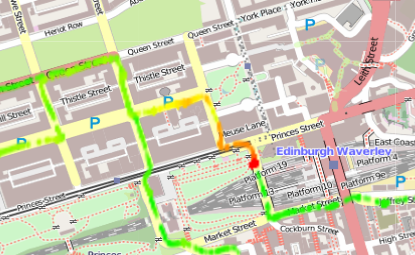
\includegraphics[width=\textwidth]{./images/StationaryPollutantBuildUp.png}
	        \caption{A map of air pollution around Edinburgh city centre. Image uses \emph{Open Street Map}.}
	        \label{fig:stationarypollutantbuildup}
	    \end{center}
	\end{figure}

	If were were to use some statistical method on a dataset similar to that seen in figure~\ref{fig:stationarypollutantbuildup}, we could estimate with some degree of certainty what the pollution levels are in areas where there are no recordings. By doing this we could produce a map similar to the one in figure~\ref{fig:zurichheatmap}.

	\begin{figure}[H]
	    \begin{center}
	        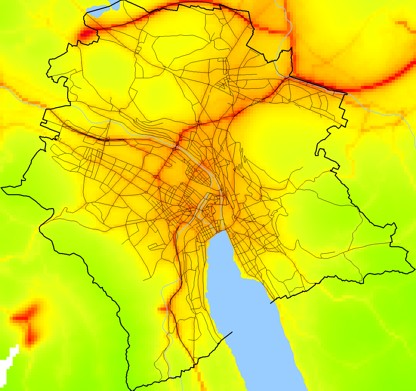
\includegraphics[width=\textwidth]{./images/zurichpm.jpg}
	        \caption{A heatmap of particulate matter in Zurich. The higher pollution levels can clearly be seen to follow transport infrastructure.~\cite{opensensezurich}}
	        \label{fig:zurichheatmap}
	    \end{center}
	\end{figure}

	
	In order to solve this problem and accurately predict the pollution levels, advanced statistical techniques, with a great deal of domain specific information, are required. Doing this would be impractical for the \emph{City of Edinburgh Council}. Instead we will employ existing tools and simpler statistical methods to help us perform this task. By using well known and understood methods, avoiding complex methods such as regression kriging~\cite{regressionkriging}, which are provided in a single tool or package, such as R or Python libraries, we will attempt to prove that this data is at least accurate enough to provide a high level overview of pollution across the city. 

	In order to validate whether our results are correct or not, we will use the freely available data from the OpenSense project and perform our analysis on this. By performing our statistical methods on a dataset from the OpenSense project we will be able to predict the pollution levels at any point in Zurich to within some degree of accuracy. By comparing the values at the same locations as a static measurement station, with the results from said measurement station, we will obtain a metric which informs us of the accuracy of the interpolation method.


	\subsection{Statistical Methods}\label{datavalidation_statisticalmethods}
		This section focuses on the various statistical methods of interpolating and extrapolating data values at arbitrary points on a grid. These methods vary in their effectiveness on different data sets, however it is important to note that none of these methods take into account data which could be viewed as extremely important in this case. An example of this is the terrain. In section~\ref{research_geostatisitcalmodelling} we discuss the effect that canyoning has on air quality readings. This effect is ignored by these models. 

		A further crucial piece of information which needs to be taken into account is that these models do not take into account temporal changes of readings. In order to use our data sets we will have to have a way of ``snapshotting'' data. A choice needs to be made for the length of time each snapshot should be. A suggestion for a rough value is 30 minutes, however experimental results will reveal the best value to use.

		%http://en.wikipedia.org/wiki/Multivariate_interpolation


		\subsubsection{Regular Grid Algorithms}\label{datavalidation_regulargrid}

			These interpolation methods require a regular grid with data points placed onto them and will calculate all missing values. In order to be able to do this we will need to place our results into ``buckets''. Buckets of around $5m^{2}$ will allow us to have a reasonable resolution for data without our calculations taking too long. The boxed area which the trams cover in Zurich is roughly 4km by 5km. This gives us a grid resolution of 800*1000, for a total of 800,000 data points. 

			\textbf{Barnes}\label{datavalidation_barnes} \\

				Barnes interpolation uses a multi-pass approach to determine the new data points. The method has found success in calculating air pressure across the United States, providing results similar to careful analysis, however it depends on the data points be reasonably uniform~\cite{barnesinterpolation}.

				No examples existed in either R or Python and so a custom implementation written in Python was created. This implementation follows the information in the original paper by Barnes and has shown success on test data sets. The algorithm works by calculating a simple distance weighted interpolation as the first result, and then iterating multiple times using a calculated error field to reduce the errors in the output. 

				One important factor in Barnes interpolation is the fact that it depends on server constants. These constants depend on the type of data being interpolated and the nature of the measurements, including the density of the measurements. As such, determining these constants is a key part of using this algorithm for interpolation. One advantage of this approach, is that we can iterate over our data set and fit it to the known measurements in order to make sure it is as accurate as possible. With this method however, we lose test data points and so cannot validate it. Experiments using this algorithm have used similar mechanisms and shown success~\cite{pmconcentrationmaps}.

				The algorithm for Barnes interpolation is as follows.

				For the first pass each known point is assigned a weight using the formula: 

				\begin{align*}
					W_{i} &= e^{-(d/R^{2})}
				\end{align*}
				
				where d is the distance between the known point and the current point to be interpolated, and R is the radius of influence. Using this weight, the initial guess of the grid points is calculated as: 
				
				\begin{align*}
					X_{g} &= \frac{\sum_{i}{W_{i}X_{i}}}{\sum_{i}{W_{i}}}
				\end{align*}

				At this point we begin our successive passes. These are defined as:

				\begin{align*}
					X'_{g} &= X_{g} + \frac{\sum_{i}{W'_{i}E_{i}}}{\sum_{i}{W'_{i}}}
				\end{align*}

				where $E_{k}$ is the difference between the estimated value and the actual value at a known point $k$ and $W'_{i}$ is defined as:

				\begin{align*}
					W'_{i} &= e^{-(d/\Gamma R)^{2}}
				\end{align*}

				with $\Gamma$ as a convergence parameter normally set in the range 0.2-0.3.

				The created Python code for this algorithm is as follows:

				\tdi{Fix this code and make it nice.}
				\inputminted[mathescape,linenos,numbersep=5pt,frame=lines,framesep=2mm]{python}{./code/barnes.py}

			\textbf{Bilinear}\label{datavalidation_bilinear} \\


			
			\textbf{Bicubic}\label{datavalidation_bicubic} \\
			
			\textbf{B\'{e}zier Surface}\label{datavalidation_beziersurface} \\
			
			\textbf{Lanczos Resampling}\label{datavalidation_lanczosresampling} \\
			
			\textbf{Delaunay Triangulation}\label{datavalidation_delaunaytriangulation} \\
			
			\textbf{Natural Neighbor}\label{datavalidation_naturalneighbour} \\
			
			\textbf{Spline Interpolation}\label{datavalidation_splineinterpolation} \\

		\subsubsection{Irregular Grid Algorithms}\label{datavalidation_irregular_grid}

			\textbf{Radial Basis Function}\label{datavalidation_radial_basis_function} \\

			\textbf{Thin Plate Spline}\label{datavalidation_thin_plate_spline} \\

			\textbf{Least-Squares Spline}\label{datavalidation_least_squares_spline} \\

		\subsubsection{Hybrid Algorithms}\label{datavalidation_hybrid_algorithms}

			%http://en.wikipedia.org/wiki/Nearest-neighbor_interpolation
			\textbf{Nearest Neighbour}\label{datavalidation_nearest_neighbour} \\

				Nearest neighbour interpolation is the simplest interpolation we will see in that it is not really interpolation at all. Instead the value of each point is the value of the closest data point we have. A na\"{\i}ve version of the algorithm in Python, with \emph{known\_points} being a list of tuples containing the co-ordinates and value of each known point, is as follows\:

				\inputminted[mathescape,linenos,numbersep=5pt,frame=lines,framesep=2mm]{python}{./code/nearest_neighbour.py}

			\textbf{Inverse Distance Weighting}\label{datavalidation_inversedistanceweighting} \\

				Inverse Distance Weighting, known as IDW, is the second simplest algorithm. Each point is a weighted average of all known points, where the weighting is the inverse of the distance. 

				Each value is calculated as follows:

				\begin{align*}
					V = \frac{\sum_{i=1}^{n}{\frac{v_{i}}{d^{p}_{i}}}}{\sum_{i=1}^{n}{\frac{1}{d^{p}_{i}}}}
				\end{align*}

				Once again, there are parameters which must be supplied to the algorithm which are data dependent. In this case the parameter is the smoothing factor. A lower smoothing factor means that the interpolated value at a known data point is closer to the value of the known data point. A higher smoothing factor makes the rate of change smaller to give a smoother graph and the cost of some interpolated points being different to known values which are nearby.

			\textbf{Kriging}\label{datavalidation_kriging} \\
		
	\subsection{Implementation}\label{datavalidation_implementation}
	\subsection{Results}\label{datavalidation_results}
	\subsection{Conclusion}\label{datavalidation_conclusion}
